\documentclass{beamer}
\usepackage{amsmath}
\usepackage{algpseudocode}
%\newcommand{\IN}{{\texttt{In}}}
%\newcommand{\OUT}{{\texttt{Out}}}
\newcommand{\IN}{{\texttt{X}}}
\newcommand{\OUT}{{\texttt{Y}}}
\newcommand{\DIM}{{\texttt{d}}}
\newcommand{\OUTSMOOTH}{{\texttt{OUT}_{\texttt{NN}}}}
\newcommand{\TWO}{\{\pm\}}
%\newcommand{\PAR}{{\texttt{Par}}}
\newcommand{\PAR}{{\texttt{P}}}

\newcommand{\GD}{{\texttt{GD}}}

\newcommand{\CO}{{\hat w}}
\newcommand{\NNW}{{\tilde w}}

\newcommand{\UC}{{\texttt{C}_{\texttt{FPFN}}}}

\newcommand{\BS}{{P_{\texttt{bs}}}}
\newcommand{\RAND}{{\texttt{rand}}}
\newcommand{\SHUFF}{{\texttt{shuff}}}

\newcommand{\TRN}{{\texttt{Train}}}
\newcommand{\TST}{{\texttt{Test}}}

\newcommand{\RKG}{{\texttt{RKG}}}

\newcommand{\PRED}{{\hat y}}%{{\texttt{Pred}}}
\newcommand{\PREDSMOOTH}{{\tilde y}}%{{\texttt{Pred}_{\texttt{NN}}}}
\newcommand{\yP}{{\hat y}}
\newcommand{\YP}{{\hat Y}}
\newcommand{\YN}{{\tilde Y}}
\newcommand{\UPD}{{\texttt{Upd}}}
\newcommand{\UPDSTEP}{{\texttt{Upd}_{\texttt{step}}}}
\newcommand{\UPDEP}{{\texttt{Upd}_{\texttt{epoch}}}}
\newcommand{\UPDFIT}{{\texttt{Upd}_{\texttt{fit}}}}
\newcommand{\Prob}{{\mathbb P}}
\newcommand{\ProbH}{{\widehat{\mathbb P}}}

\newcommand{\XYEP}{{\texttt{Z}_{\texttt{epoch}}}}
\newcommand{\XB}{{\texttt{X}_{\texttt{B}}}}
\newcommand{\YB}{{\texttt{Y}_{\texttt{B}}}}

\newcommand{\FP}{{\texttt{FP}}}
\newcommand{\FN}{{\texttt{FN}}}
\newcommand{\CFP}{{\texttt{C}_\FP}}
\newcommand{\CFN}{{\texttt{C}_\FN}}
\newcommand{\FPE}{{\widehat{\texttt{FP}}}}
\newcommand{\FNE}{{\widehat{\texttt{FN}}}}
\newcommand{\Fp}{\widetilde{\texttt{FP}}}
\newcommand{\Fn}{\widetilde{\texttt{FN}}}
\newcommand{\FPB}{{\texttt{FP}_B}}
\newcommand{\FNB}{{\texttt{FN}_B}}
\newcommand{\FPT}{{\texttt{FP}_\oplus}}
\newcommand{\FNT}{{\texttt{FN}_\oplus}}

\newcommand{\CTHRESH}{{\texttt{C}}_{\texttt{FPFN}}}

\title{Constraint awareness for binary classification}
\subtitle{George Lee}
\begin{document}
\begin{frame}
\titlepage
\end{frame}

\section{Setup and motivation}
\begin{frame}
\frametitle{Setup}
\begin{itemize}
\item
  Broad problem setting: for a pair of \textbf{random variables} (RVs) $z_\omega=(x,y)$ taking values in $\IN\times\OUT$, infer a \textbf{class label} $y\in\OUT$ based on the \textbf{feature} $x\in\IN$.
\item
  Focus on \textbf{binary classification}, $y_\omega\in\TWO$
\item
  Depending on context $\IN$ might be $\left(\texttt{float}\right)^{\DIM_\IN}$ or $\mathbb R^{\DIM_\IN}$
\item Initial setting is
    \begin{itemize}
\item
  Offline: we are provided with an $N$ row dataset $Z=(X,Y)$ with $(X_i,Y_i)\in\IN\times\OUT$ for $1\leq i\leq N$.
\item
  iid: rows are assumed to be drawn \textbf{independently and identically distributed}, $(X,Y)\sim_{\texttt{iid}}(x,y)$.
\item
  $p=\Prob(y=+)$ can be estimated by $\hat p=\ProbH(Y=+)=\tfrac{\#Y=+}{\#Y}$ for $N\gg p^{-1}$.
    \end{itemize}
\end{itemize}
\end{frame}
\begin{frame}
\frametitle{Is class imbalance worth resampling over?}
\begin{itemize}
\item
  We focus on techniques for \textbf{imbalanced} data, ie $p\ll1$: we assume that there are enough samples to learn the features of $Y$ to some tolerance.
\item
  Current problem: investigate alternatives to computationally expensive training data \textbf{resampling} schemes $(SMOTE^*,TOMEKS^*,\cdots)$
\item
Offline validation by randomly splitting $\{1,\cdots,N\}=\TRN\sqcup\TST$ into train and test sets.
\item
  UNSW-NB15: no appreciable gains from resampling compared to training using a regression model, when an appropriate threshold is selected based on train dataset
\end{itemize}
\end{frame}
\begin{frame}
\frametitle{Note on iid offline setting}
\begin{itemize}
  \item
    Without these assumptions the problem might be as hard as any prediction problem we might pose in ml, since the output of any model can be represented as asequence of bits.
  \item
    Useful for initial algorithm benchmarking, but hard to beat SOTA regression techniques in this relatively well understood setting.
    Fundamentally want to develop techniques that may be used in an online setting, where updates to a model will have to be made in response to an evolving sequence of costs for errors and time sensitive user defined constraints
\end{itemize}
\end{frame}
\begin{frame}
\frametitle{Regression based classification}
\begin{itemize}
\item
%  In our context a \textbf{learning method} (LM) with inputs in $\IN$ and outputs in $\OUT$ with parameter space $\PAR$ is a tuple $(\PRED,\UPD)$ consisting of \textbf{prediction} and \textbf{update} rules
  A learning algorithm on $\IN\times\OUT$ parameterised by $\PAR$ consists of prediction and update maps
\begin{gather*}
  \PRED:\PAR\times\IN\rightarrow\OUT\text{ and}\\
  \UPD:\PAR\times\left(\IN\times\OUT\right)^{<\infty}\rightarrow\PAR.
\end{gather*}
\item
  Want to find a model where $\OUT$ takes discrete parameters, but based on an underlying regression where $\OUT$ takes continuous values
\end{itemize}
\end{frame}
\begin{frame}
\frametitle{Classifiers from regressors}
\begin{itemize}
\item
  Fix parameters $w\in\PAR$
\item
  Many binary classifiers modelling RVs $(x,y)$ are based on regression models
\item
  feature $x\rightsquigarrow$ regression inference $\PREDSMOOTH\rightsquigarrow$ binary class label $\PRED$
\item
  Respective parameters for the overall model then are $w=(\NNW,\CO)$
\item
  The continuous-valued prediction $\PREDSMOOTH(\NNW,x)$ is classified according to a cutoff hyperparameter $\CO$:
  $$
  \PRED(\PREDSMOOTH,\CO)=\begin{cases}+\text{ if }\tilde y>\CO,\\-\text{ otherwise.}\end{cases}
  $$
\item
  When dataset or batch $(X,Y)$ fixed write $\YN_i=\PREDSMOOTH(X_i)$ and $\YP_i=\yP(\YN_i)$ for the binary and continuous inferences respectively.
\end{itemize}
\end{frame}
\begin{frame}
\frametitle{Error rates, estimation and relaxation}
  \begin{itemize}
\item
In this setting only need to infer one bit of information $y\in\TWO$ at a time
\item
Accordingly, two possible types of errors
\item
Fix a batch $B\subseteq\{1,\cdots,N\}$ on which to estimate statistics.
\begin{gather*}
  \FP=\Prob(\yP>y),~\FN=\Prob(\yP<y),\\
  \FPE_B=\ProbH_B(\YP>Y),~\FNE_B=\ProbH_B(\YP<Y),\\
  \Fp_B=\tfrac1{\#B}\sum_{i\in B:Y_i=-}\YN_i\text{ and }\Fn_B=-\tfrac1{\#B}\sum_{i\in B:Y_i=+}\YN_i.
\end{gather*}
\item
  $\FP$ and $\FN$ are the model's (true) \textbf{false positive} and \textbf{false negative} rates
\item hats: binary estimate: best indication of the true rates, but not differentiable
\item tildes: "surrogate error" or "likelihood" depending on perspective
\end{itemize}
\end{frame}
\begin{frame}
\frametitle{Regression approach}
\begin{itemize}
\item
  For a fixed batch, reducing $\Fp$ and $\Fn$ will reduce $\FP$ and $\FN$
\item
  The NN $\PREDSMOOTH$'s raw gradient updates can be expected to move $\YN$ in the correct direction at a rate that depends on the marginal distribution $\mathbb P(x|y)$.
\end{itemize}
\end{frame}
\begin{frame}
\frametitle{User defined constraints}
\begin{itemize}
\item
  Aim: fit models that meet \textbf{user defined constraints} on the false positive and false negative rates.
\item
  Algorithm needs an objective function to optimise: user needs to select one
\item
  Estimates of objective might not be immediately amenable to gradient descent algorithms required for NN training
\item
  $\FP$ and $\FN$ are two probabilities, and we seek to reduce both according to a precise definition of their relative importance.
\end{itemize}
\end{frame}
\begin{frame}
\frametitle{Constraining the constraints}
\begin{itemize}
\item
  Parameter selection should be explainable
\item
  Constraint is in terms of continuous RVs $\FP$ and $\FN$ but constraint satisfaction measured will be scored by binary performance $\FPE_\TST$ and $\FNE_\TST$.
\item
  We need to find a continuous objective to train a NN model
\item
  Example: demanding that a model have error rates below fixed targets $\FPT,\FNT\in(0,1)$ is equivalent to requiring that $C(\FP,\FN)<0$ for the map
  $$
    C(s,t)=\texttt{max}(\tfrac s{\FPT},\tfrac t{\FNT})-1.
  $$
\item
  Higher $\FP$ and $\FN$ is always bad, any objective
\item
  Want to decide on tradeoff in rigorous manner
\end{itemize}
\end{frame}
\begin{frame}
\frametitle{Choosing a cost I}
\begin{itemize}
\item
  Explainable choice for user defined objective: constraint $C(\FP,\FN)$ will take the form of a $\textbf{cost}$
\item
  Old, well understood, but seems intrinsically better than many common statistics\cite{ferrerno}:
\begin{itemize}
\item
  Can be scaled to be independent of priors and for cost of 1 to be eqiuivalent to the best guesses that always guesses the more likely class
\item
  Simple, intuitive gradient profile
\item
  For a fixed regression model this continuous objective is backed by theory, this and gradient descent methods suppresing importance of loss function geometry anull the need to search for the perfect loss
\end{itemize}
\end{itemize}
\end{frame}
\begin{frame}
\frametitle{Choosing a cost}
\begin{itemize}
\item
  Simplest case user knows costs of false positives and false negatives $\rightsquigarrow$ use $C(s,t)=s\CFP+t\CFN$.
\item
  Requiring a user to specify a notion of their costs and gains as a function of $\FP$ and $\FN$ is necessary to define the problem being solved.
\item
The only effect of $C$ is to define the relative importance of reducing $\FP$ versus $\FN$ at each point on the unit square
\end{itemize}
\end{frame}
\begin{frame}
\frametitle{Choosing a cost II}
\begin{itemize}
  \item
    If as in previous slide costs known in advance, apply gradient update method to $\UC(\Fp,\Fn)=C_\FP\Fn+C_\FN\Fn$ to target an actual solution to the problem.  However, can generalise to broader scenarios
  \item
    If the costs can only be approximated as RVs with finite expectations, it is optimal to minimise using the expactations of those costs
  \item
    If nothing is known, then optimising BCE equivalent to minimising AUC/ROC/etc
  \item
    In the offline setting, this may suggest searching for other objectives is unnecessary
\end{itemize}
\end{frame}
\begin{frame}
\frametitle{Architecture vs loss selection}
\begin{itemize}
  \item
    Should we focus on loss choice or architecture in model design?
  \item
    There is a duality between NN architecture and loss - a loss which is a function of $\Fp$ and $\Fn$ can be seen as another layer
\end{itemize}
\end{frame}
\begin{frame}
\frametitle{Choice of architecture vs loss}
\begin{itemize}
\item
Models are commonly trained to minimise a loss which in some way represents how far predictions are from the target with no regard for the class, for example

\begin{gather*}
  L_{L^2}(B)=\sum_{i\in B} |\YP_i-Y_i|^2,\text{ or, if }\OUT_{\texttt{NN}}\subseteq(0,1),\\
  \texttt{BCE}(B)=-\tfrac1{\#B}\left(\sum_{i\in B_+}\log(\hat Y_i)+\sum_{i\in B_-}\log(1-\hat Y_i)\right)
\end{gather*}
\item
These choices of loss function place similar importance on making the model's predictions close to the actual value for every data point, and one may use them interchangably by rescaling the last layer of the NN appropriately.
\end{itemize}
\end{frame}
%\begin{frame}
%\frametitle{Gradient descent}
%\begin{itemize}
%\item
%  For a NN with fixed forward pass implementation $\PREDSMOOTH$ and cutoff $\CO$ there are many possible choices of routines which can be composed and iterated as we please to make new ones.
%\item
%  Fix a sufficiently well behaved loss function and gradient descent routine
%    \begin{gather*}
%      L:(\OUTSMOOTH\times\TWO)^{<\infty}\rightarrow\mathbb R\text{ and}\\
%      \GD:\PAR_\GD\times\PAR_w\times\PAR_w\rightarrow\PAR_\GD\times\PAR_w.
%    \end{gather*}
%\item
%A single update step $\UPDSTEP$ is given by
%\begin{algorithmic}[0]
%\Function{$\UPDSTEP$}{$P,\XB,\YB$}
%  \State $(P_\GD,P_w)\gets\GD(P_\GD,P_w,\partial_w(L(\PRED(P,\XB),\YB)))$
%  \State\Return $P$
%\EndFunction.
%\end{algorithmic}
%\end{itemize}
%\end{frame}
%\begin{frame}
%\frametitle{Epochs and fitting algorithms}
%\begin{itemize}
%\item
%A fitting method $\UPDFIT$ typically repeatedly iterates the update step over the randomly batched training set, repeatedly calling an epoch learning method
%\item
%   For fixed random key generator $\RKG$ and batched shuffling routine $\SHUFF$
%   % \begin{gather*}
%   %   \RKG:\PAR_\RAND\rightarrow\PAR_\RAND\text{ and}\\
%   %   \SHUFF:\mathbb N\times\PAR_\RAND\times\left(\IN\times\OUT\right)^{<\infty}\rightarrow\left(\IN\times\OUT\right)^{(<\infty)\times(<\infty)},
%   % \end{gather*}
%  such a routine is given by
%\item
%\begin{algorithmic}[0]
%  \Function{$\UPDEP$}{$P$,$X$,$Y$}
%  \State batched$\gets\SHUFF(\BS,P_\RAND,(X_i,Y_i)_i)$
%  \ForAll{$(\XB,\YB)\in$ batched}
%  \State $P\gets\UPDSTEP(P,\XB,\YB)$
%  \EndFor
%  \State $P_\RAND\gets\RKG(P_\RAND)$
%  \State\Return $P$
%  \EndFunction
%\end{algorithmic}
%\end{itemize}
%\end{frame}
%\begin{frame}
%\frametitle{Constraint aware training I: class weighting}
%\begin{itemize}
%\item
%  Relative rates of false positives and false negatives of the previous loss functions may be adjusted after training by a routine that chooses an appropriate $\CO$.
%\item One may move between the loss functions describe above by rescaling the last layer of the NN appropriately.
%  However, one may choose a loss $\CO$ which depends on target classes and instead make gradient descent steps that reduce the value of $C$ throughout the training process.
%  Updates on the last layer of a network's bias have the effect of controlling the relative rates.
%\item
%  Seek to minimise an intuitive/explainable choice of loss function $L(B)=-\beta\sum_{i\in B_+}\hat Y_i+\tfrac1\beta\sum_{i\in B_-}\hat Y_i$.
%  These losses are all increasing functions of the errors: neural networks are capable of learning nonlinear relationships in any case, and modern gradient descent methods also go some way toward mitigating the differences between different choices of loss.
%\end{itemize}
%\end{frame}
\begin{frame}
\frametitle{Cost choice influences resulting FP-FN tradeoff without posthoc thresholding}
\begin{itemize}
\item
  BCE is often used for training, but cost less ubuquitous
\item
  The functions learned are related, but targetting one specific cost reduces dimensions of the problem by 1 and may force the algorithm to concentrate on learning points near a certain likelihood of being in a classs rather than worring about AUC
\end{itemize}
\end{frame}
\begin{frame}
\frametitle{Cost choice influences resulting FP-FN tradeoff without posthoc thresholding}
\begin{itemize}
\item
Focus on malicious communication detection per UC2, where typically $p\ll 1$ and false positives may be far more tolerable and have less serious consequences than false negatives.
\item
  Training directly on cost does force a corresponding payoff
  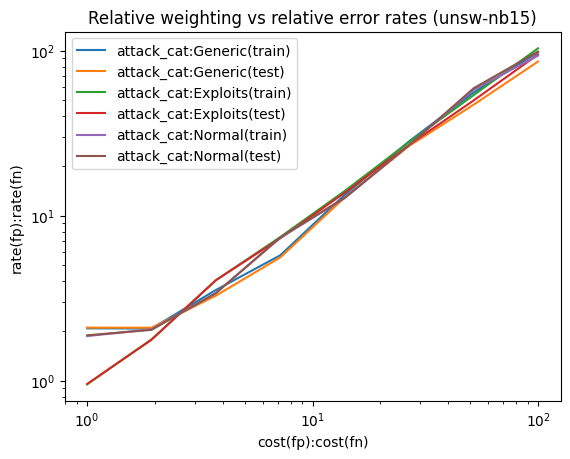
\includegraphics[scale=0.35]{fpfn_tradeoff_effect.png}
%\item
%A python class was developed to benchmark classification algorithms over a range of possible false positive and false negative targets
%\item
%$\texttt{ModelEvaluation}$ provides an interface for comparison of multiple classification algorithms
%\item 
%In order to benchmark binary classification performance over a range of problems, a dataset with greater than two classes may be provided: models are then trained to distinguish one class from many.
%
%\item
%$\texttt{ModelEvaluation}$ instantiates $\texttt{MultiTrainer}$s, each of which trains models with fixed hyperparameters but with varying end times, class labels and target error rates.
\end{itemize}
\end{frame}

%\begin{frame}
%\frametitle{Is resampling beneficial?}
%\begin{itemize}
%\item
%Class weighting appears to achieve similar results while avoiding an extra step.
%unsw-nb15:
%\end{itemize}
%\end{frame}
%\begin{frame}
%\end{itemize}
%\frametitle{...But are we learning likelihoods?}
%\begin{itemize}
%\item
%Consider the case where $g$ takes values in $[0,1]$, so that the threshold is to be chosen from $(0,1)$.
%\item
%A model is said to be \textbf{perfectly calibrated} if $\Prob(y=+|g(x)=t)=t$ for any $t\in[0,1]$.
%In this case, the output of the model can be understood as a probability that the label belongs to the positive class.
%\item
%This can be measured using the test set, for example by checking that over small intervals $[t-\delta,t+\delta]$ we have
%$$
%\frac{\#\{i\in\texttt{TEST}: |g(X_i)-t|<\delta\text{ and }Y_i=+\}}{\#\{i\in\texttt{TEST}: |g(X_i)-t|<\delta\}}\approx t.
%$$
%\end{itemize}
%\end{frame}
%\begin{frame}
%\frametitle{...But are we learning likelihoods? Continued}
%\begin{itemize}
%\item
%One should bear in mind that being well calibrated is no measure of the predictive abilities of a model!
%Note that if $g(x)=p$ for all values of $x$, then the model is perfectly calibrated but useless for classification.
%\item
%If $g$ is not perfectly calibrated, then it is often still possible to rescale its values $\tilde g(x)=h(g(x))$ such that $\tilde g$ is ``close'' to being perfectly calibrated.
%\end{itemize}
%\end{frame}
%\begin{frame}
%\frametitle{A criterion for the benefits of constraint aware binary classification}
%\begin{itemize}
%\item
%Idea: if we are able to find a good calibration $\tilde g$ of a model $g$, then the model has effectively learned likelihoods.
%\item
%In this case, we should be skeptical of the idea that we benefitted from a ``constraint aware'' training process, since we can still choose a threshold to meet any desired compromise between the false positive and false negative rates
%\end{itemize}
%\end{frame}

\bibliography{imbalanced}{}
\bibliographystyle{plain}

\end{document}
